%-----------------------------------------------------------------------------%
%                                                                             %
%    K A P I T E L   6                                                        %
%                                                                             %
%-----------------------------------------------------------------------------%

\chapter{Online Stabilization of the Planned Motions}\label{c6}
This chapter presents a two-step validation of the physical compliance of the planned motions where an online stabilization is applied to track the optimal trajectories. At first, we proof the stability of the motions in a real-time physics simulation. Following this, we explore the feasibility of the motions in real-world experiments on a full-size humanoid robot.    

\section{Validation in Real-Time Physics Simulation}\label{sec:OnlineSimulation}
This section investigates the stability of the planned motions in a physics simulator by applying an online stabilization based on joint space position control to track the trajectories obtained from \gls{OC}. To begin with, an overview of the simulation setup is given, then the tracking results of the planned motions are discussed. 

\subsection{Simulation Setup}
The optimal motions are tested in the dynamical simulation environment PyBullet \cite{coumans2016pybullet}. PyBullet is an open-source framework for robotics simulation that allows fast computation of rigid-body dynamics along with collision detection. The focus of PyBullet is to minimize the simulation-to-reality ('sim-to-real') gap, which is, despite constantly improving robot models, still a major problem in real-world experiments. To this end, the simulation in the simulator is setup in a similar way the motions would be tested o a real robot, namely interpolating the trajectories and closing the loop on joint position level.

The control loop on the real system (see \cref{sec:OnlineExperiments}) is running at a frequency of 1000Hz. The generated bipedal walking variants and highly-dynamic movements presented in \crefrange{c4}{c5} are generated with with an discrete \gls{OC} formulation at 30Hz and 10Hz, respectively. To this end, the optimal trajectories are interpolated with a cubic spline in order to realize an up-scaling of the reference data to 1000Hz.  

The control architecture consists of a simple PD-controller on joint space level. The controller is supposed to track both position and velocity reference trajectories with the standard PyBullet parameters in a real-time loop running at 1000Hz. In this real-time simulation, the same URDF robot model is used as in the Crocoddyl framework, including similar maximal motor torques. Furthermore, the parameters of the rigid contact models have been aligned between both frameworks to ensure comparability.

\subsection{Results}
Following up, we investigate the capabilities of the presented control architecture for tracking the planned motions. To this end, we study the control tracking performance for the dynamic walking gait (\cref{sec:BipedSimulation}) and a highly-dynamic forward jump (\cref{sec:HighlySimulation}).

\subsubsection{Dynamic Walking}
To begin with, we analyze the motion tracking for dynamic walking gait. \cref{fig:walkDynamic_pybulletTracking} shows the tracking performance of the joint level control architecture. The reference trajectories from \gls{OC} are visualized as solid lines, while the resulting trajectories of the real-time physics simulation are shown as dotted lines. It can be seen that the controller follows the optimal trajectories fairly good. Small deviations can be seen around two seconds, which accounts for the lift off phase for the second robot step. This effect can be explained by the apparent abrupt change in the joint space, but is found to be marginal for the overall tracking performance. 
\begin{figure}[h!]
\centering	
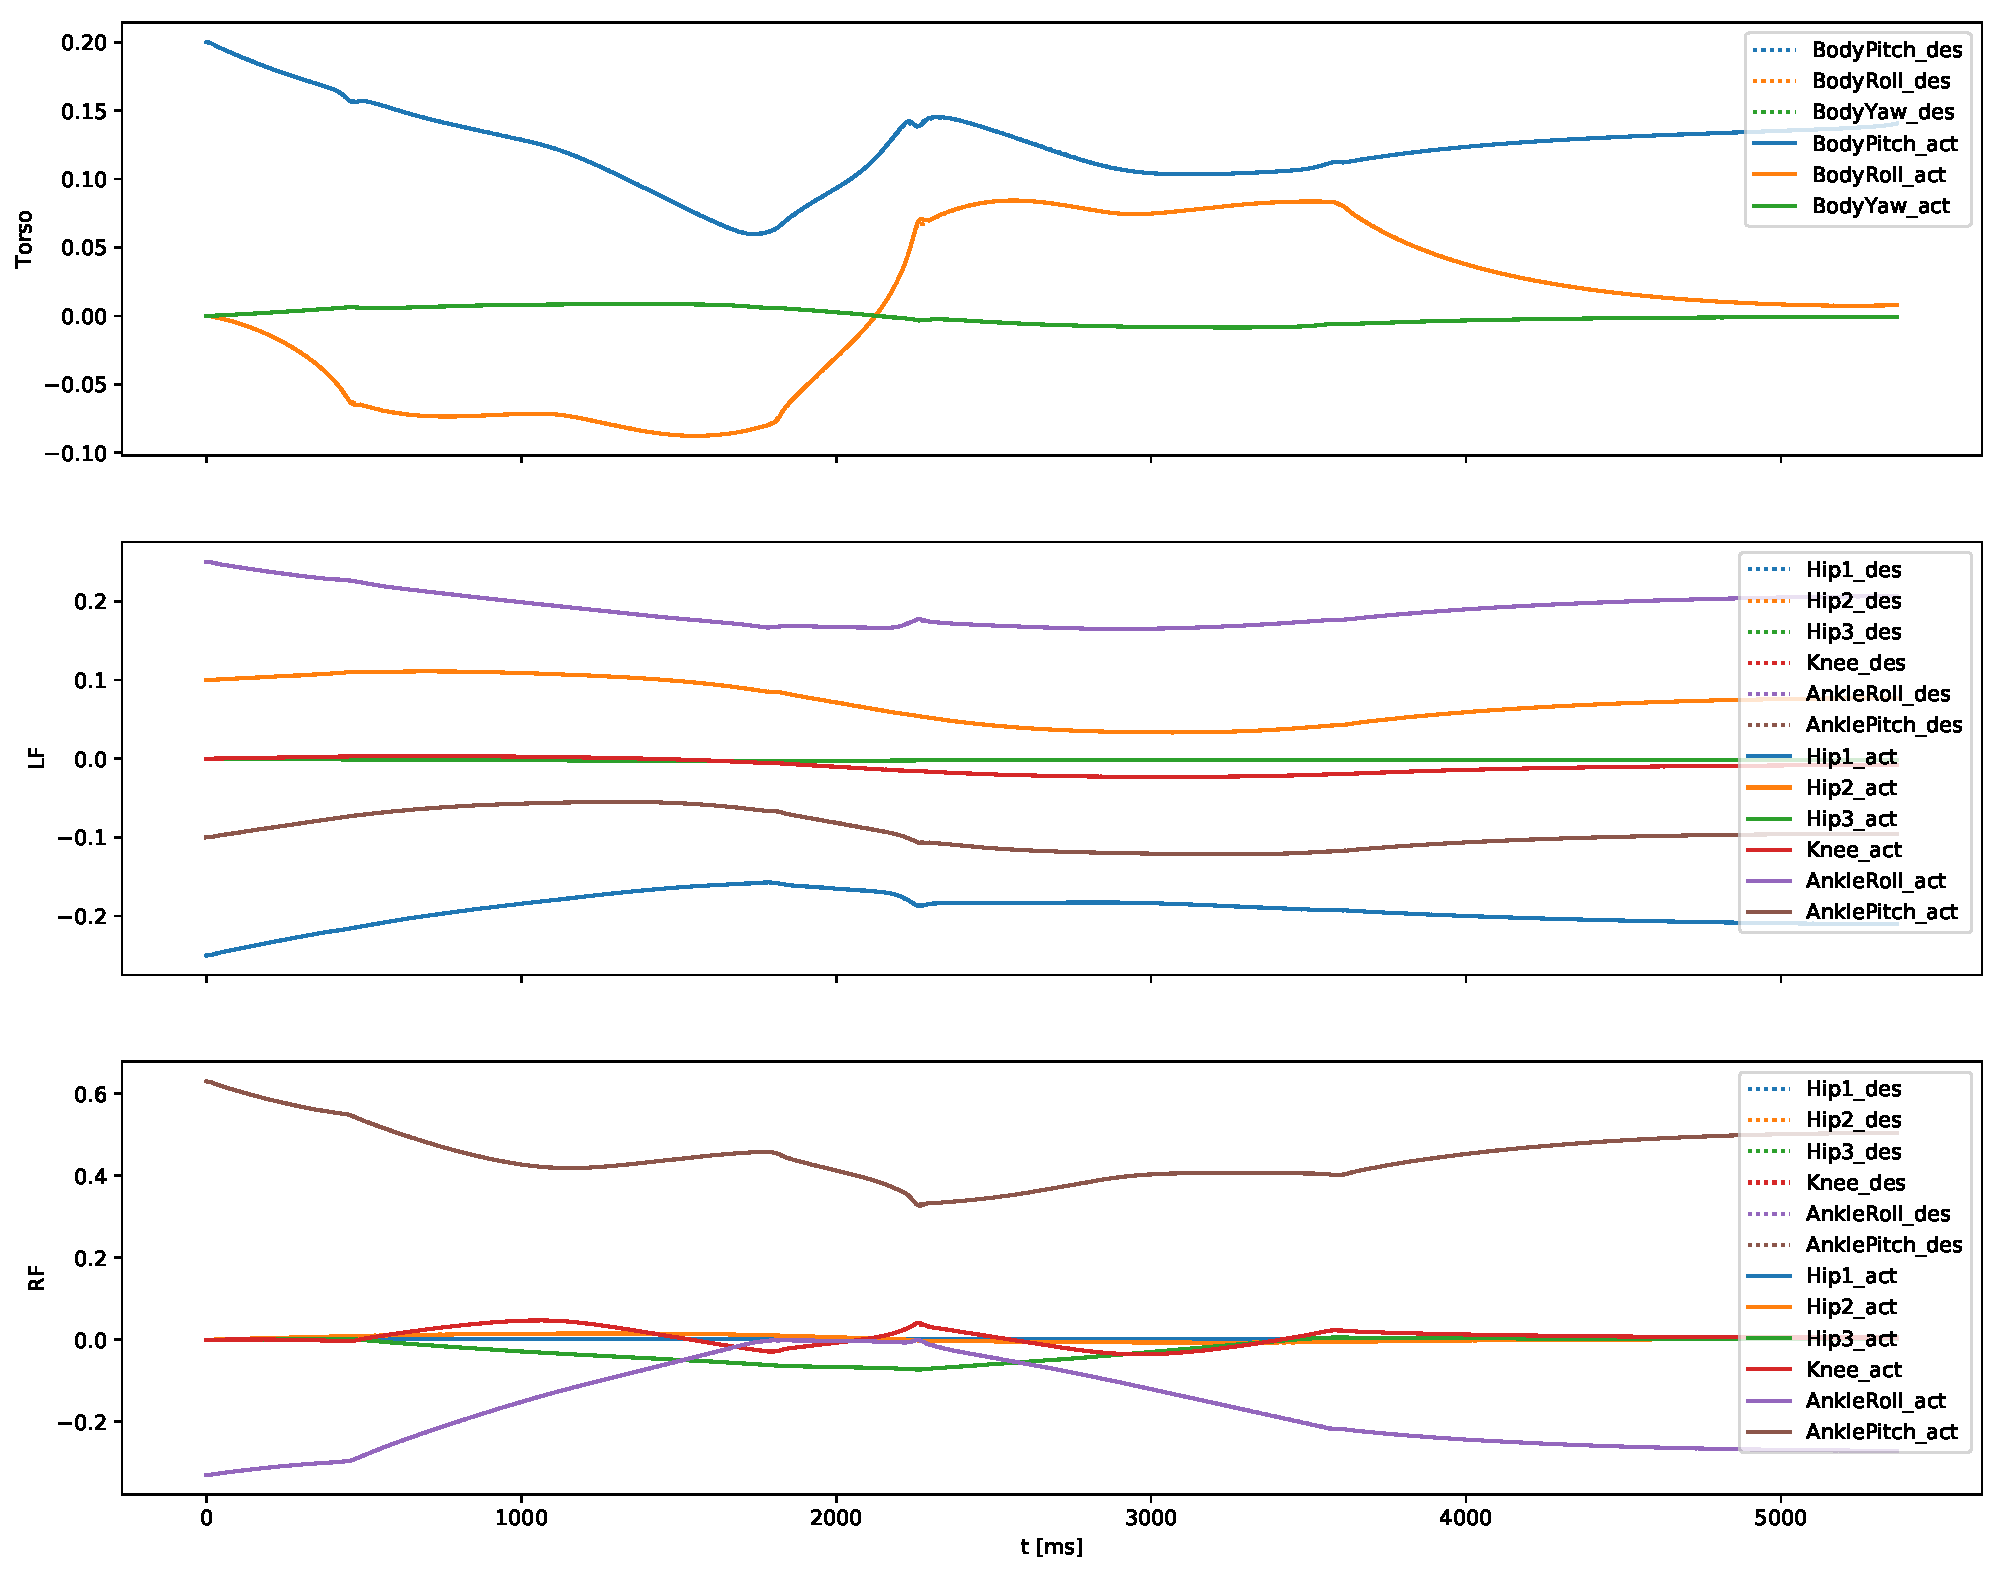
\includegraphics[width=1\textwidth]{fig/walkDynamic/pybullet/pybulletTracking}
\caption{Control tracking performance on joint level for the dynamic walking gait.}
\label{fig:walkDynamic_pybulletTracking}
\end{figure}

As introduced previously, the control architecture is solely based on joint space position and velocity level. Although the tracking performance is good, this does not proof for the stability of the motions. Similar to the definition of robot tasks, also the evaluation of the motions should be pursued in task space. To this end, \cref{fig:walkDynamic_pybulletBase} monitors the according motion of the floating base. As can be seen, the floating base deviates about $\pm$ 10mm in x and y-direction , as well as $+$ 5mm in z-direction. 
\begin{figure}[h!]
\centering	
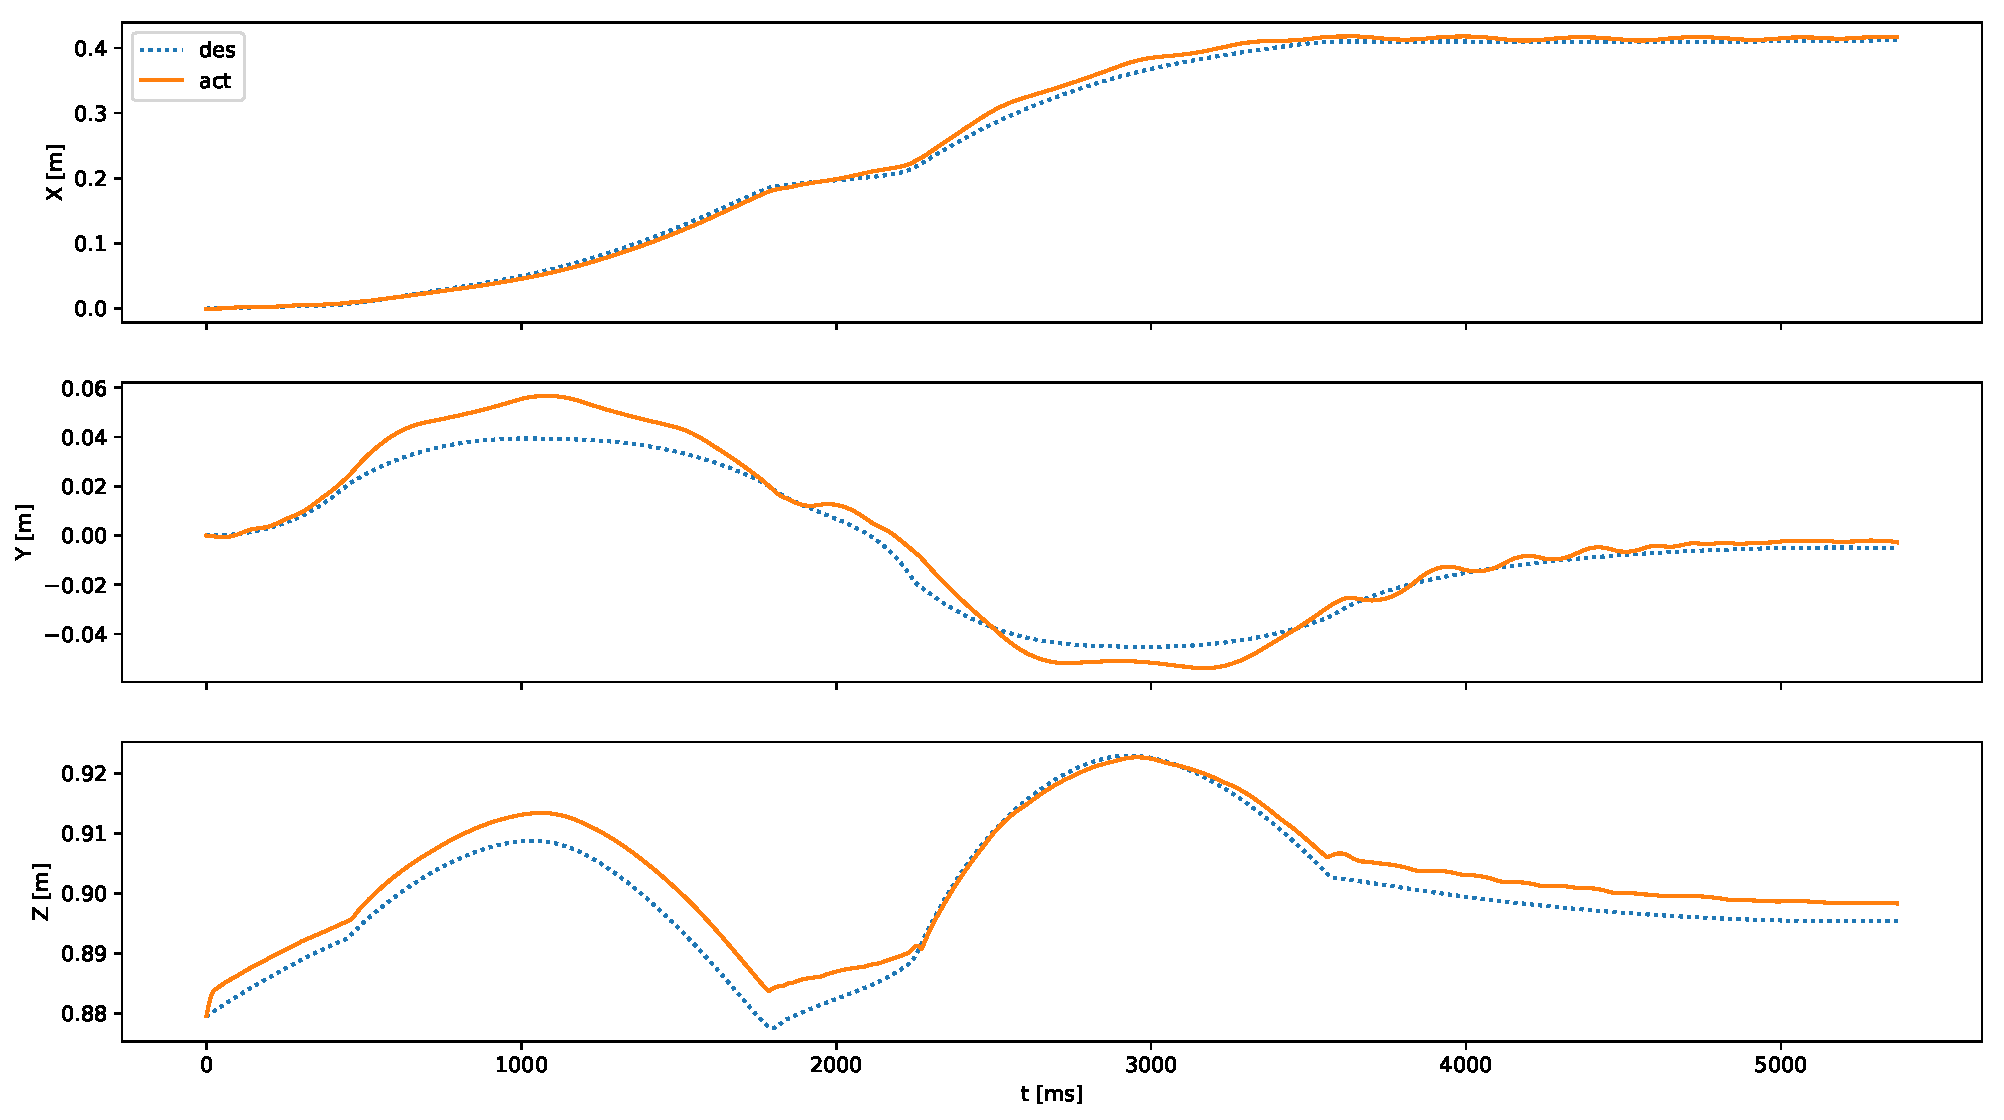
\includegraphics[width=1\textwidth]{fig/walkDynamic/pybullet/pybulletBase}
\caption{Motion of the floating base resulting from joint space control for the dynamic walking gait.}
\label{fig:walkDynamic_pybulletBase}
\end{figure}

In this context, it is important to notice that no controller tracks these task space quantities. Instead, they are merely the result of the joint space control performance. The largest deviations in task space occur during the first step and the according impact in the first two seconds of the motions. It becomes evident that these task space errors do not correlate to the peaks discussed on joint space level. Furthermore, one can observe oscillations in the stabilization phase at the end of the motion. This effect can be attributed to the fact that the systems slightly starts to swing after the second impact. This behavior could be compensated e.g. with a dedicated control in task space instead of joint space. 

Overall it can be stated that the dynamic walking motion can be successfully stabilized by the proposed control approach. 

\subsubsection{Forward Jumping}
To identify the limits of the control approach, we now study the online stabilization for a highly-dynamic forward jump (\cref{sec:HighlySimulation}). In addition to the previously discussed dynamic walking, the jumping task introduces new challenges for the controller in terms of speed and robustness that will be investigated in the following.  

\ref{fig:jumpForward_pybulletTracking} shows the tracking performance of the joint level control architecture for the forward jump. In contrast to the case of dynamic walking, the joint space controller reveals larger tracking deviations. This is especially true for the most dynamic part of the motion, namely the acceleration of the base and finally the takeoff around 300-400ms. Large deviations can be especially seen for body pitch, and the knee joints, which turned out to be crucial for highly-dynamic movements. 

\begin{figure}[h!]
\centering	
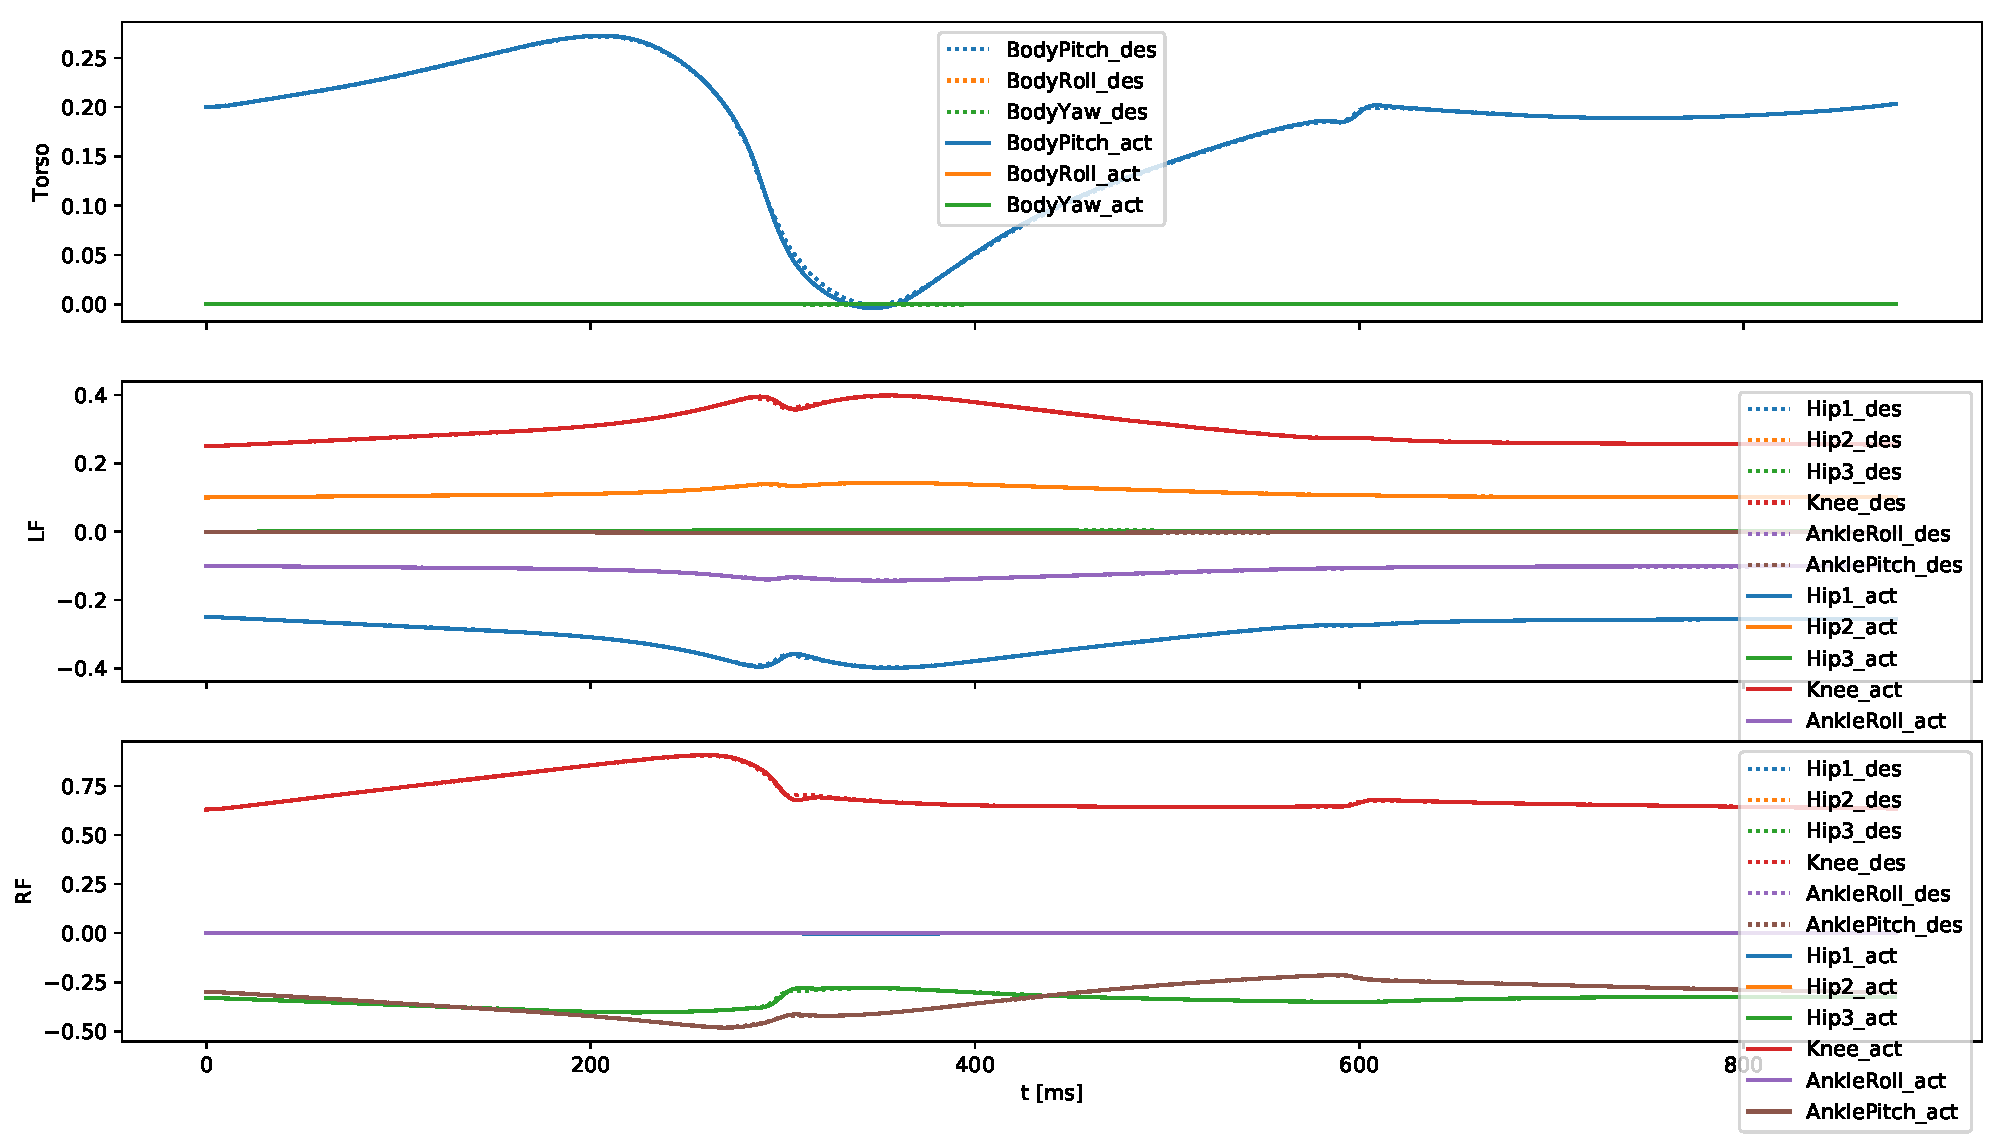
\includegraphics[width=1\textwidth]{fig/jumpForward/pybullet/pybulletTracking}
\caption{Control tracking performance on joint level for a forward jump.}
\label{fig:jumpForward_pybulletTracking}
\end{figure}


\begin{figure}[h!]
\centering	
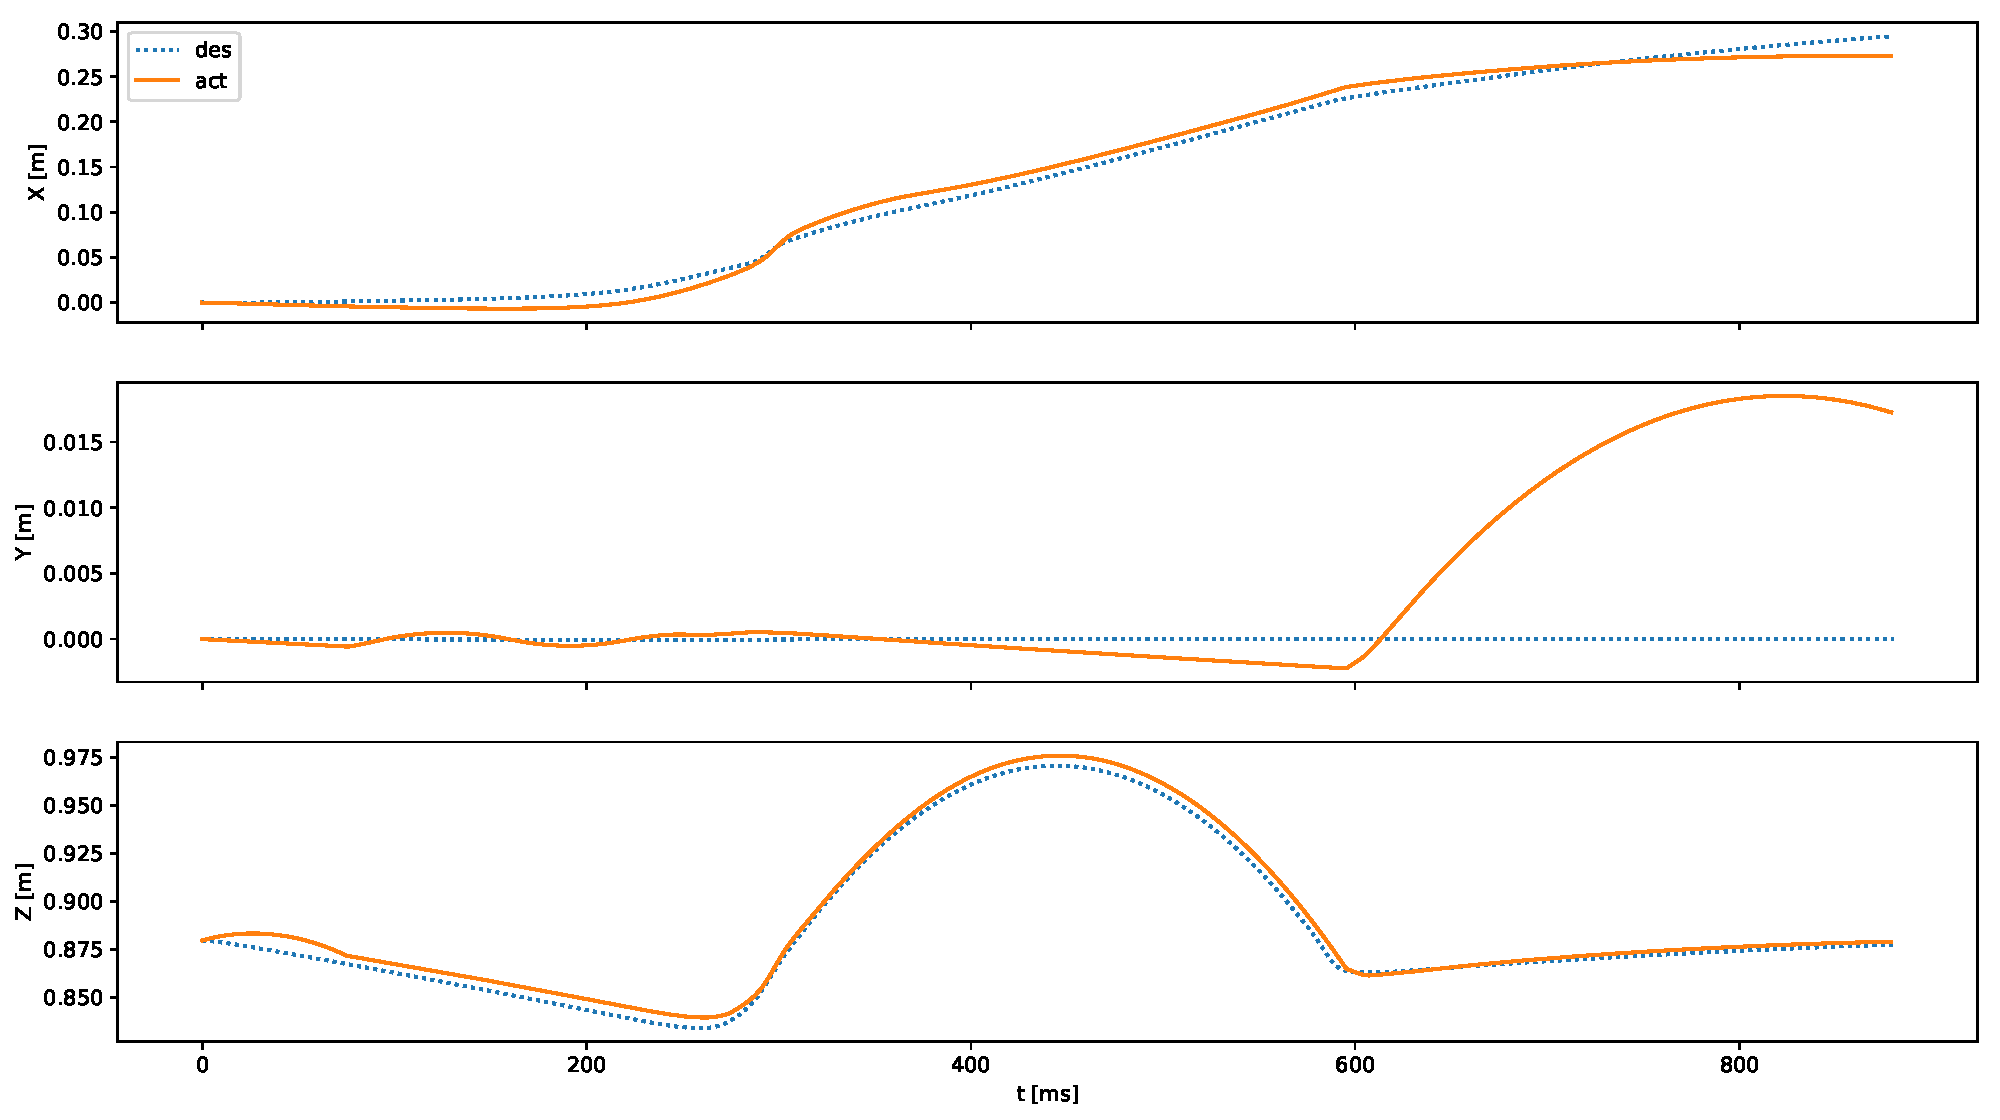
\includegraphics[width=1\textwidth]{fig/jumpForward/pybullet/pybulletBase}
\caption{Motion of the floating base resulting from joint space control for a forward jump.}
\label{fig:jumpForward_pybulletBase}
\end{figure}

In company with these findings, \cref{fig:jumpForward_pybulletBase} monitors the motion of the (uncontrolled) floating base resulting from the joint space control performance. As becomes evident, the deviations in tasks space are also much higher compared to the dynamics walking case. While the height of the floating base is reasonable, the x-position shows tracking errors of about $\pm$ 5cm. Errors of this magnitude inevitably lead to instability of the movement to be performed. In this case, the strong deviation in task space causes the robot to tilt around the rear edge of the foot after the touchdown. 

Consequently, it turned out that a mere control on a joint space basis is not sufficient to track highly dynamic movements, but is indeed appropriate to stabilize a dynamic walking gait in real-time. 


\section{Validation in Real-World Experiments}\label{sec:OnlineExperiments}
This section investigates the stability of the planned motions in real-world experiments on the full-size humanoid robot RH5 (see \cref{subsec:RH5}). Analogously to the validation in PyBullet, the goal is to track the \gls{OC} trajectories with a joint space online stabilization on the real system. 

A total of four experiments are conducted. The primary goal is to examine whether the presented control architecture is sufficient to follow the static and dynamic walking trajectories (see \crefrange{c4}{c5}). For a dedicated root cause analysis we test two additional motions on the real-system, namely one-legged balancing and a sequence of dynamic squat movements. The respective goal is to identify potential model deviations and to study the capabilities of the real-time controller.

Based on the simulation results from the last section, highly dynamic movements are not evaluated on the real system in the context of this thesis. As discussed in the last section, these motions definitely require more advanced control algorithms in task space due to the dynamic nature of the movement. 

The rest of this section is structured as follows. First, an overview of the experimental setup with the involved components is presented. Following up, the experiments are presented and discussed with respect to the tracking performance and the stability of the motion.

\subsection{Pipeline}\label{subsec:Pipeline}
The foundation for the experiments are the motion data generated offline with the proposed whole-body \gls{TO}. The planned motions are then tracked in real-time with a joint space online stabilization on the real system. An overview of the experimental pipeline is given in \cref{img:experimentalSetup}. In the following, details on the involved components are provided. 
\begin{figure}[h]
\centering	
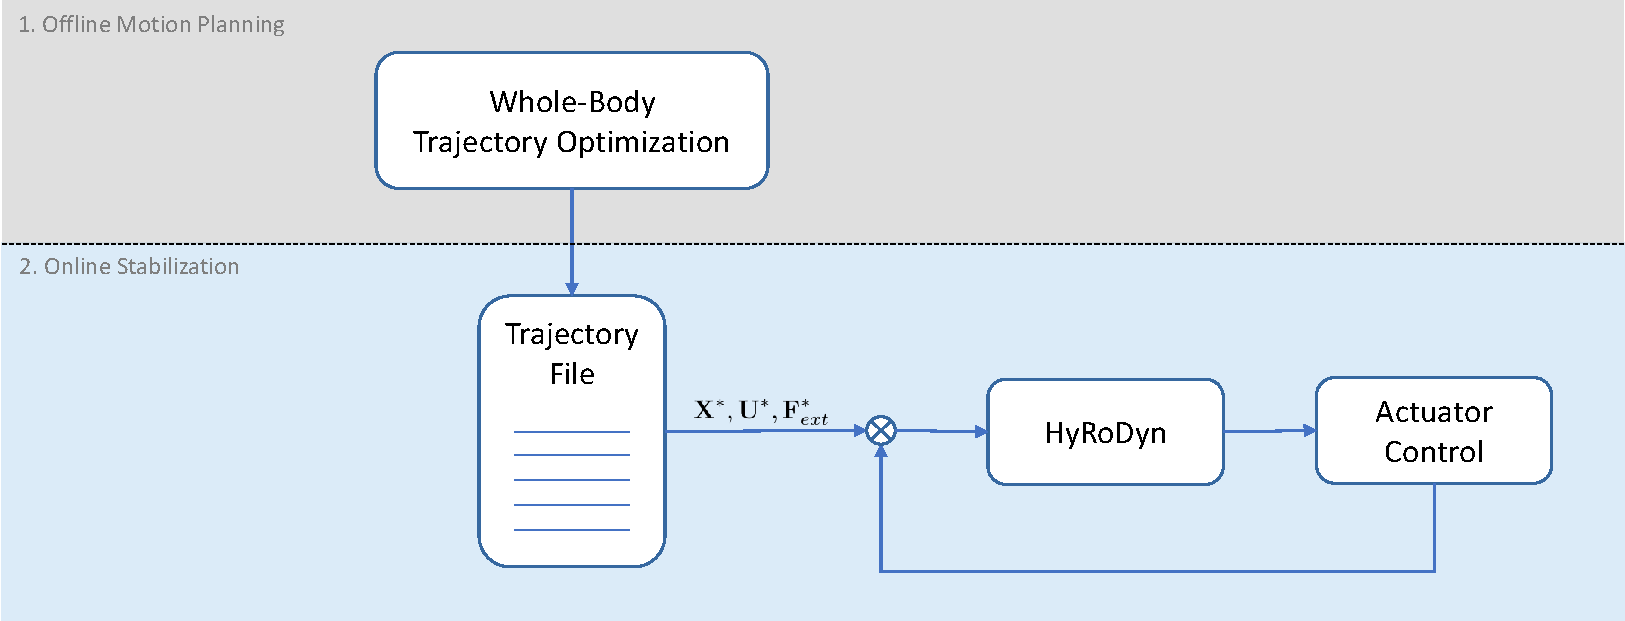
\includegraphics[width=1\textwidth]{img/experimentalSetup1}
\caption{Overview about the experimental pipeline.}
\label{img:experimentalSetup}
\end{figure}
%Trajectory File
The presented motion planning approach computes inherently balanced motions that are concisely captured in an appropriate file. This trajectory file contains the optimal state trajectories $\myM{X}^*=[\bq^*,\bv^*]$, optimal control inputs $\myM{U}^*$ and the resulting contact wrenches $\myM{F}_{\text{ ext}}^*$ acting on the feet. In order to minimize the computational effort in the real-time loop, the file already encompasses data discretized to the desired frequency of 1kHz. As in the PyBullet validation, the trajectories are interpolated using cubic splines in order to ensure smoothness and derivability. 

%HyRoDyn motivation
As introduced in \cref{subsec:RH5}, the novel RH5 humanoid robot contains multiple parallel mechanisms in order to achieve a high dynamic performance, superior stiffness and payload-to-weight ratio. This leads to the presence of various closed loops and hence a series-parallel hybrid robotic system, which are difficult to model and control. In most multi-body dynamics libraries, e.g. RBDL \cite{felis2017rbdl} and OpenSim \cite{delp2007opensim}, these loop closure constraints are solved numerically. HyRoDyn (Hybrid Robot Dynamics), is a recently presented modular software framework for solving the kinematics and dynamics of these type of series-parallel hybrid robots analytically, leading to improved accuracy and computational performance \cite{kumar2018hyrodyn}.

%Abstract vs Full Model
The planned motions are computed based on a serialized robot model. For dynamic real-time control, using this simplified model turned out to be sufficient, although the accuracy is reduced \cite{kumar2019model}. Nevertheless, the problem remains on transforming the results from the independent joint space, to the actuation space. In the context of this thesis, HyRoDyn is used to map the trajectories generated for the serialized robot model to compute the forces of the respective linear actuators.

%Framwork Consistencies
Consistency of the frameworks involved in the motion planning and control pipeline is an indispensable prerequisite for the following up experiments. Hence, \cref{app:Consistency} provides a brief verification of the notability compliance between HyRoDyn and Pinocchio \cite{carpentier2019pinocchio}, which is used inside Crocoddyl for computation of robots dynamics and their analytical derivatives. 

%Control+Rock
Low-level actuator controllers are utilized to compensate deviations from the reference trajectories. Analogously to the PyBullet validation, this control approach uses a cascaded feedback of position, velocity and an additional current control loop. 
HyRoDyn, as well as the low-level control of the RH5 robot is implemented using the Robot Construction Kit (Rock) middleware \cite{joyeux2013rock}, which is based on the Orocos Real Time Toolkit and forms the software backbone of the RH5 humanoid robot. 

\subsection{Experiments}
We conduct a total of four experiments, gradually incorporating a new level of difficulty (see \cref{tab:experiments}), that are introduced in the following.
\begin{table}[t]
\centering
\caption{Overview about the difficulty of the conducted experiments.}
\begin{tabular}{lcccc}
\hline
& Balancing & Static Walk & Fast Squats & Dynamic Walk\\ \hline
Surface Contacts & \greencheckmark  & \greencheckmark & \greencheckmark & \greencheckmark \\
Base motion & \greencheckmark  & \greencheckmark & \greencheckmark & \greencheckmark \\
Swingleg motion & \greencheckmark  & \greencheckmark & \redxmark & \greencheckmark \\
Step sequence & \redxmark  & \greencheckmark & \redxmark & \greencheckmark \\
Impacts & \redxmark  & \greencheckmark & \redxmark & \greencheckmark \\
Dynamic forces & \redxmark  & \redxmark & \greencheckmark & \greencheckmark \\
%Non-flat terrain & \redxmark  & \redxmark & \redxmark & \redxmark \\
Flight-phases & \redxmark  & \redxmark & \redxmark & \redxmark \\
\hline
\quad\quad Success & \greencheckmark  & (\greencheckmark) & \greencheckmark & \redxmark \\ \hline
\end{tabular}
\label{tab:experiments}
\end{table}
\subsubsection{Experiment I: One-Leg Balancing}
The goal of this first experiment is to test the ability of the control architecture to track a slow balancing task. The quasi-static motion consists of three phases as visualized in \cref{exp:balancingSnaps}. From a stable pose in \gls{DS} (a), shift the \gls{CoM} above the left foot (b), lifting the right foot slightly up (c) and down (d) and returning back to the initial pose (e).
\begin{figure}[h!]
\begin{subfigure}{.2\textwidth}
	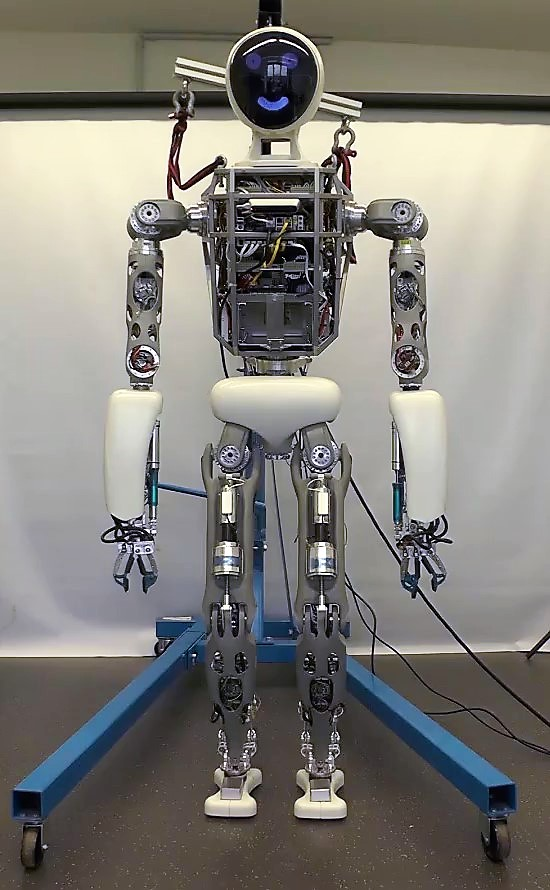
\includegraphics[width=.95\linewidth]{experiments/balancing/snaps/1}
	\end{subfigure}%
\begin{subfigure}{.2\textwidth}
	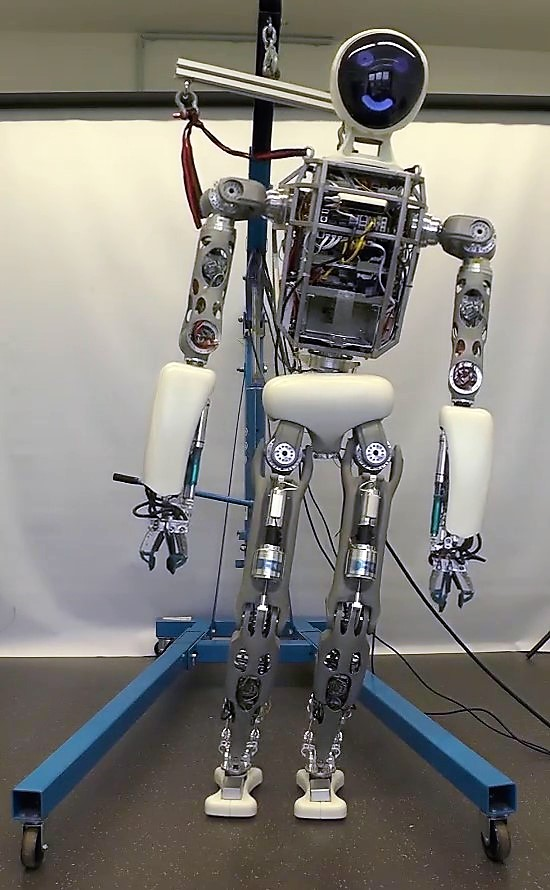
\includegraphics[width=.95\linewidth]{experiments/balancing/snaps/2}
\end{subfigure}%
\begin{subfigure}{.2\textwidth}
	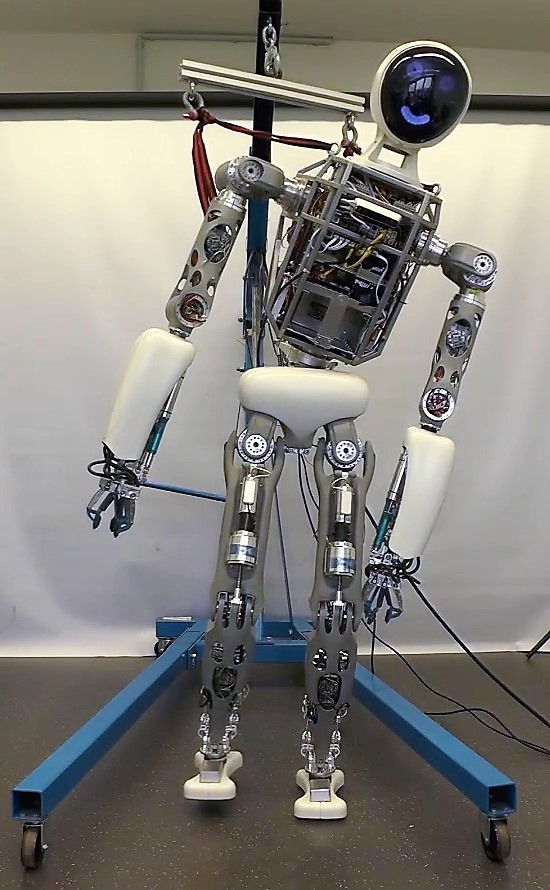
\includegraphics[width=.95\linewidth]{experiments/balancing/snaps/3}
	\end{subfigure}%
\begin{subfigure}{.2\textwidth}
	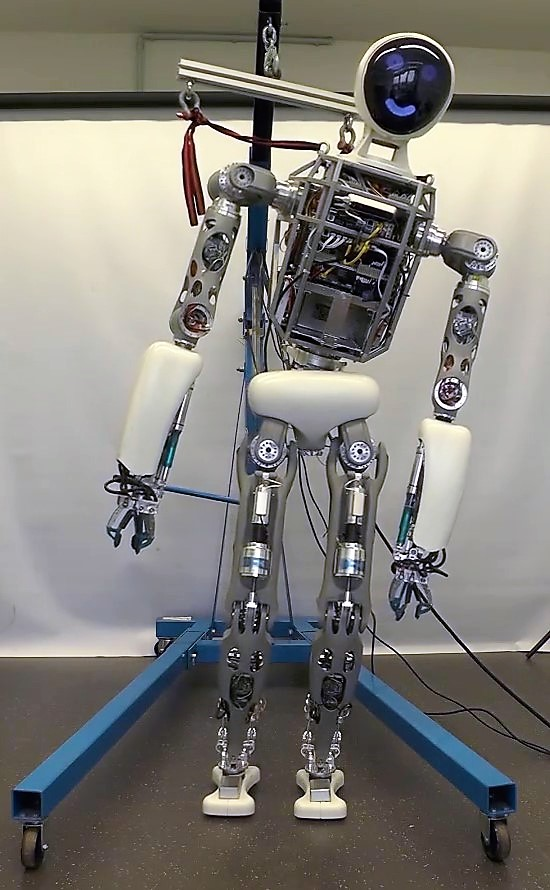
\includegraphics[width=.95\linewidth]{experiments/balancing/snaps/4}
\end{subfigure}%
\begin{subfigure}{.2\textwidth}
	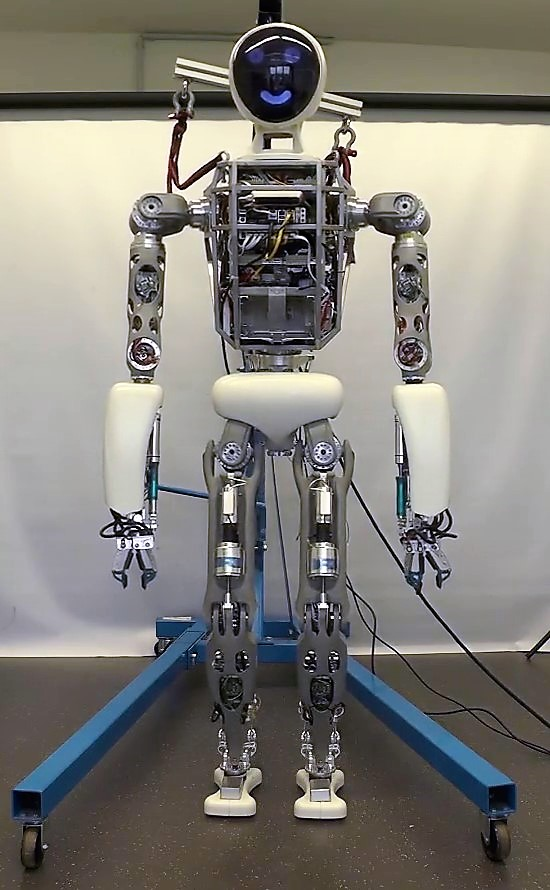
\includegraphics[width=.95\linewidth]{experiments/balancing/snaps/5}
	\end{subfigure}%
\caption{Experiment I: One-leg balancing.}
\label{exp:balancingSnaps}
\end{figure} 

\subsubsection{Experiment II: Static Walking}
The second experiment deals with a stabilization of the static walking pattern discussed in \cref{sec:BipedSimulation} (see \cref{exp:staticWalkingSnaps}). The objective of this test is to analyze the effect of more difficult swing-leg motions, a step sequence of two steps and the effect of impacts. 
\begin{figure}[h!]
\begin{subfigure}{.2\textwidth}
	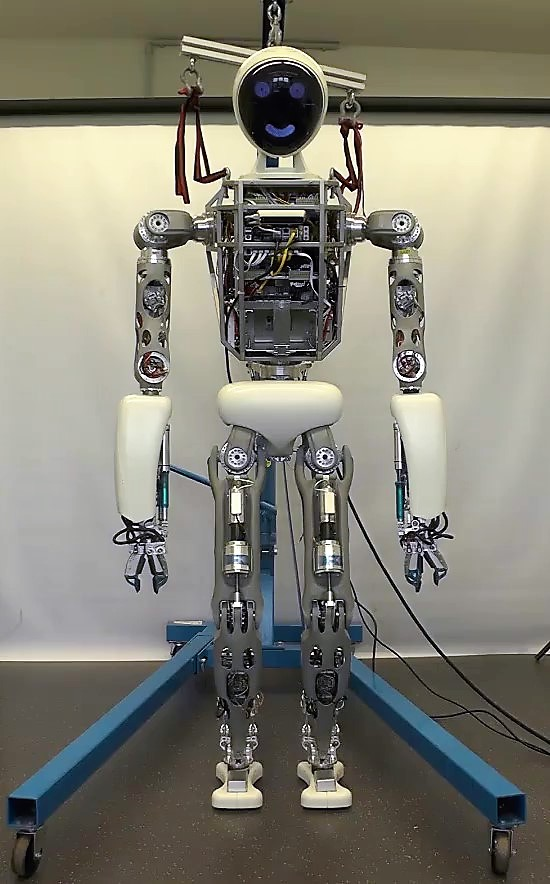
\includegraphics[width=.95\linewidth]{experiments/walkStatic/snaps/1}
	\end{subfigure}%
\begin{subfigure}{.2\textwidth}
	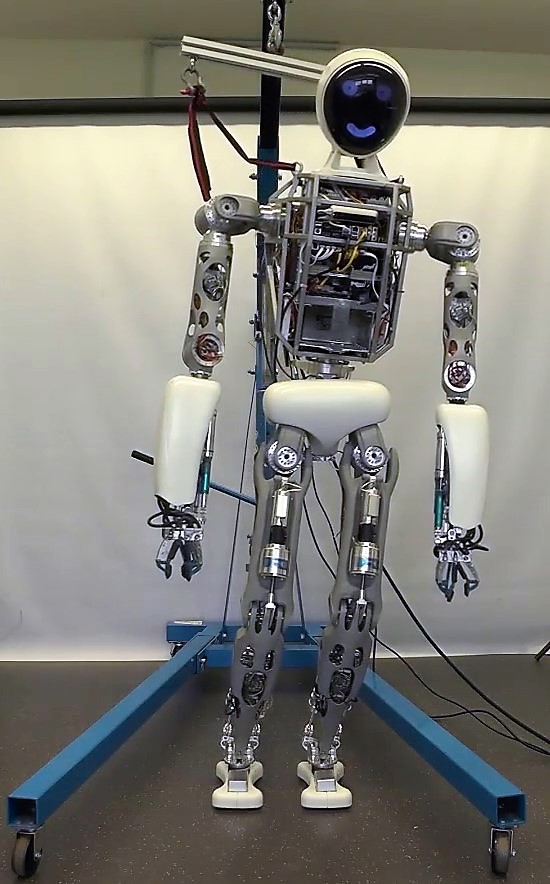
\includegraphics[width=.95\linewidth]{experiments/walkStatic/snaps/2}
\end{subfigure}%
\begin{subfigure}{.2\textwidth}
	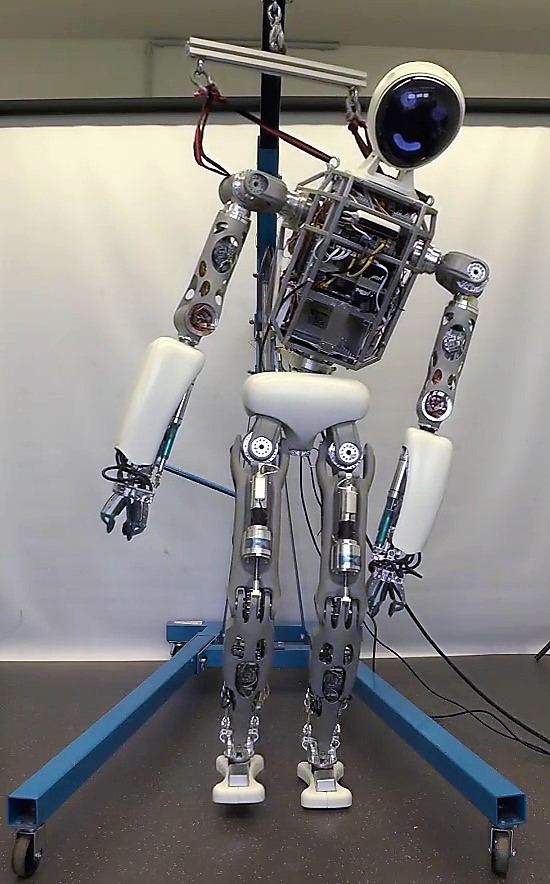
\includegraphics[width=.95\linewidth]{experiments/walkStatic/snaps/3}
	\end{subfigure}%
\begin{subfigure}{.2\textwidth}
	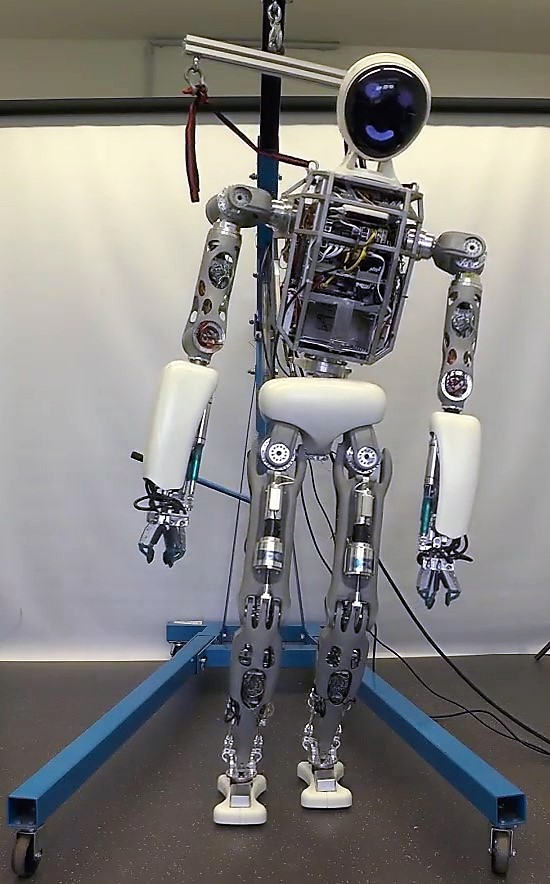
\includegraphics[width=.95\linewidth]{experiments/walkStatic/snaps/4}
\end{subfigure}%
\begin{subfigure}{.2\textwidth}
	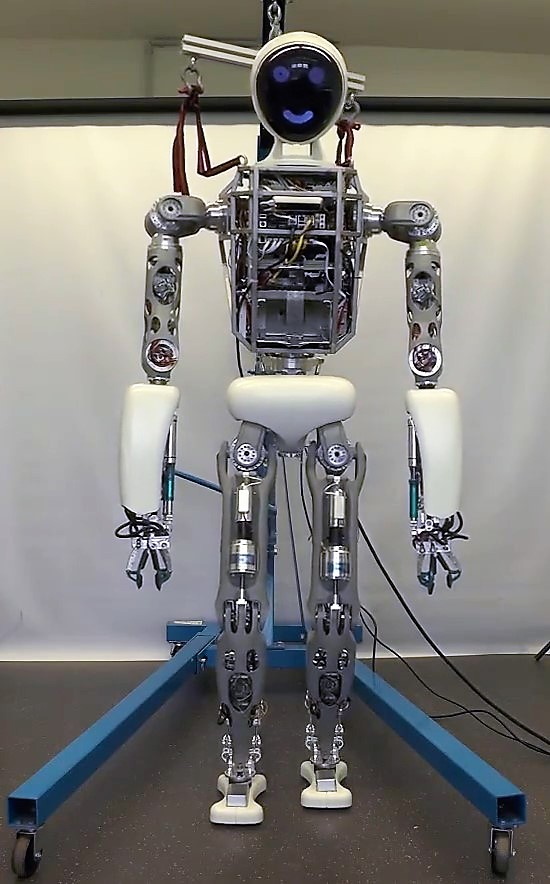
\includegraphics[width=.95\linewidth]{experiments/walkStatic/snaps/5}
	\end{subfigure}%
\caption{Experiment II: Static walking.}
\label{exp:staticWalkingSnaps}
\end{figure} 

\subsubsection{Experiment III: Fast Squats}
The objective of this third experiment is to evaluate the tracking performance in the context of a dynamic motion. In contrast to the first two motions, the fast squatting experiment (see \cref{exp:squatSnaps}) involves dynamic forces acting on the robot resulting from a fast vertical base movement in the range of 15cm within two seconds. Analogously to the multiple forward jumps (see \cref{sec:BipedSimulation}), the motion is composed of a sequence of three \gls{OC} problems that are solved sequentially (see \cref{eqn:optimizationProblemSequence}). This experiment can be seen as preliminary test for dynamic walking following in the next experiment.   
\begin{figure}[h!]
\begin{subfigure}{.14\textwidth}
	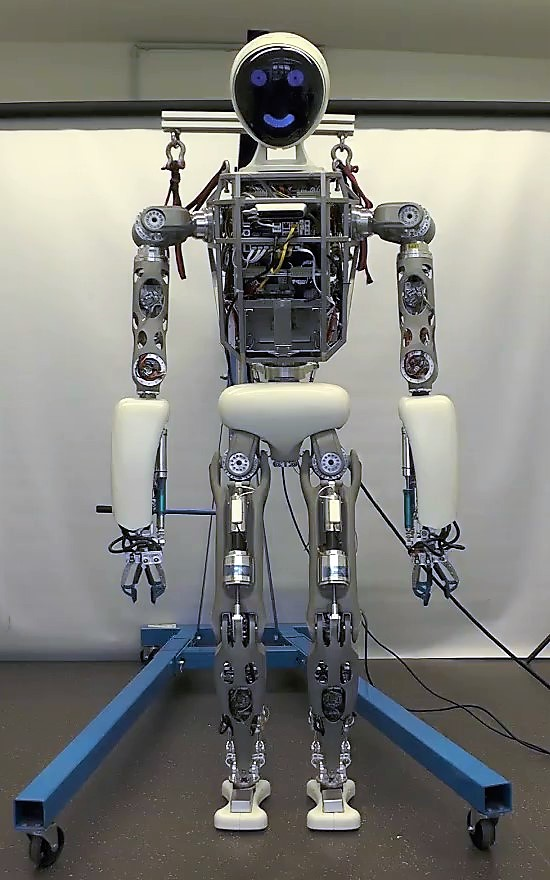
\includegraphics[width=.95\linewidth]{experiments/squats/snaps/1}
	\end{subfigure}%
\begin{subfigure}{.14\textwidth}
	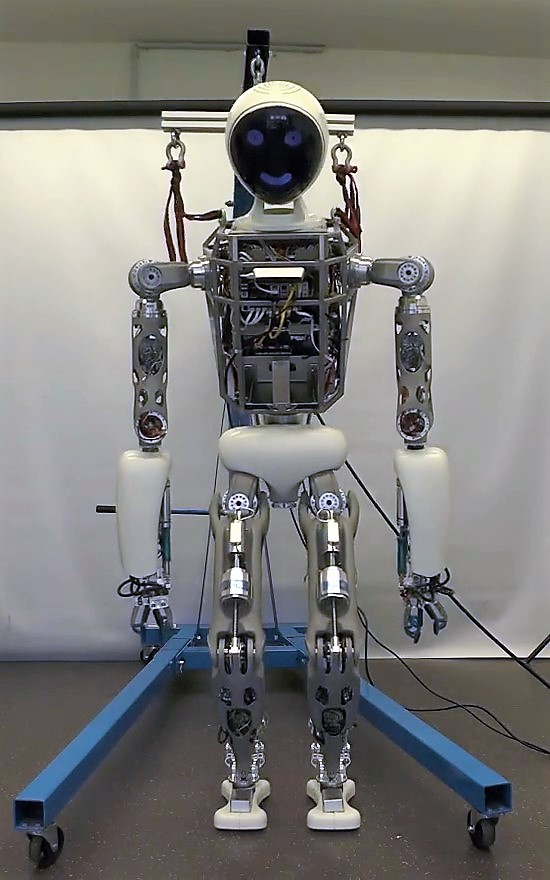
\includegraphics[width=.95\linewidth]{experiments/squats/snaps/2}
\end{subfigure}%
\begin{subfigure}{.14\textwidth}
	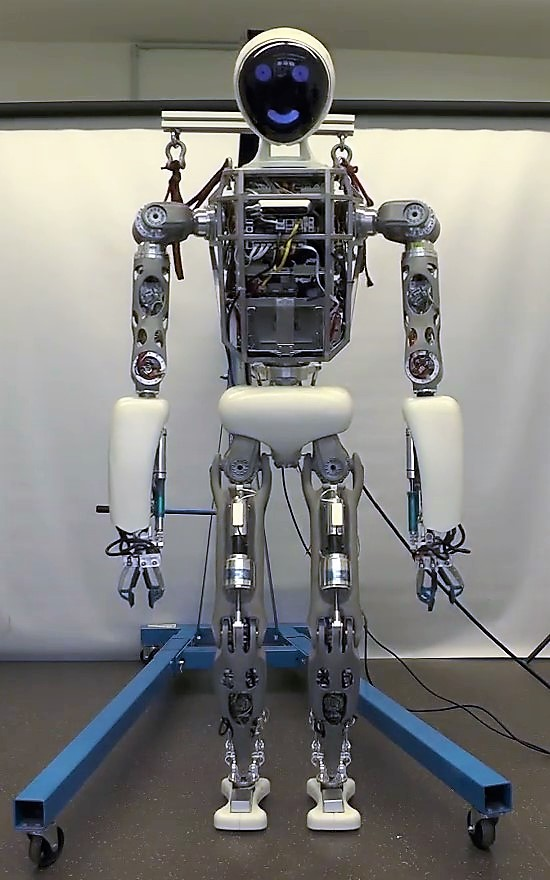
\includegraphics[width=.95\linewidth]{experiments/squats/snaps/3}
	\end{subfigure}%
\begin{subfigure}{.14\textwidth}
	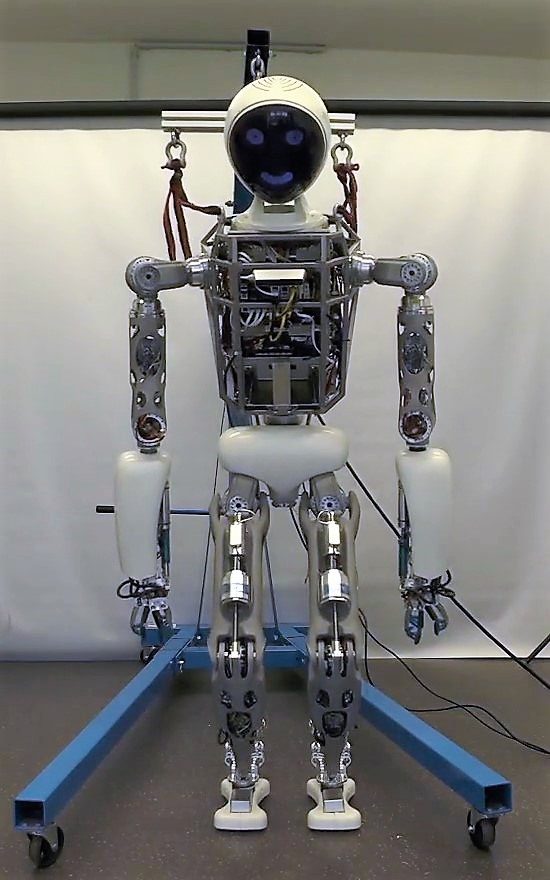
\includegraphics[width=.95\linewidth]{experiments/squats/snaps/4}
\end{subfigure}%
\begin{subfigure}{.14\textwidth}
	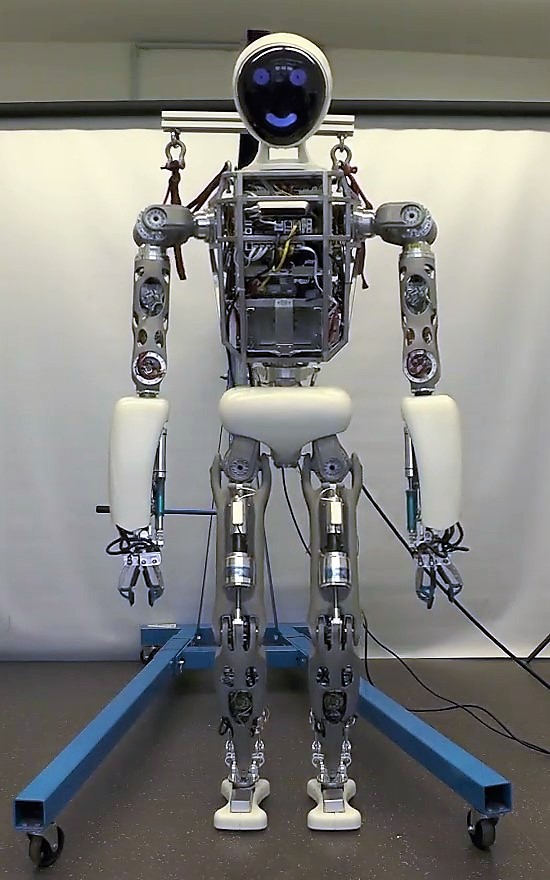
\includegraphics[width=.95\linewidth]{experiments/squats/snaps/5}
	\end{subfigure}%
\begin{subfigure}{.14\textwidth}
	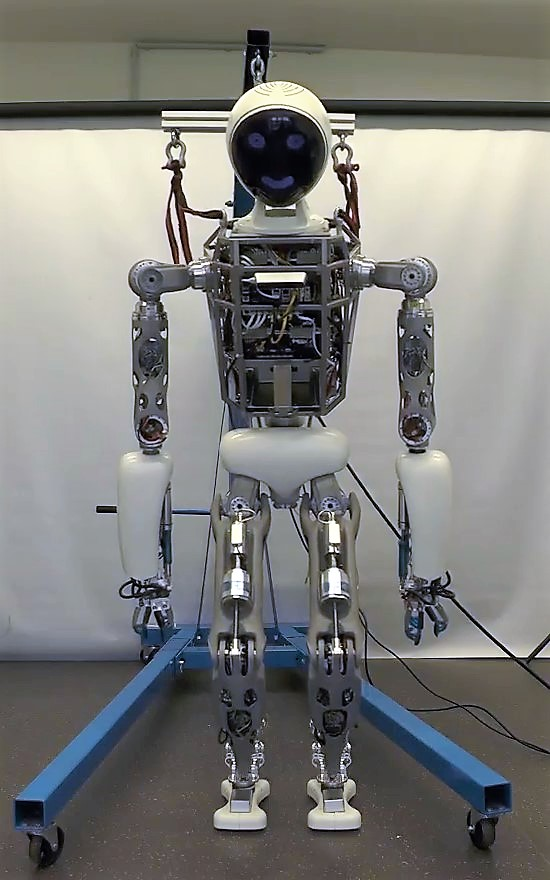
\includegraphics[width=.95\linewidth]{experiments/squats/snaps/6}
	\end{subfigure}%
\begin{subfigure}{.14\textwidth}
	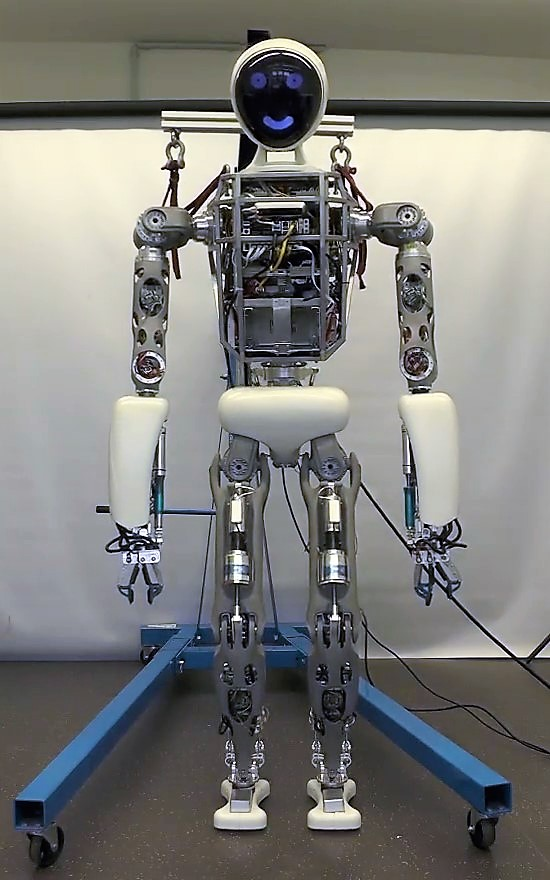
\includegraphics[width=.95\linewidth]{experiments/squats/snaps/7}
	\end{subfigure}%
\caption{Experiment III: Sequence of fast squats.}
\label{exp:squatSnaps}
\end{figure} 

\subsubsection{Experiment IV: Dynamic Walking}
This experiment investigates the capabilities of the online stabilizer to follow the dynamic walking gait trajectories presented in \cref{sec:BipedSimulation} (see \cref{exp:dynamicWalkingSnaps}). From a perspective of complexity, it combines both the challenges of static walking, namely dedicated swing-leg motions, step sequence and impacts, with the difficulty of dynamic forces acting on the robot as explored with the fast squats experiment.
\begin{figure}[h!]
\begin{subfigure}{.2\textwidth}
	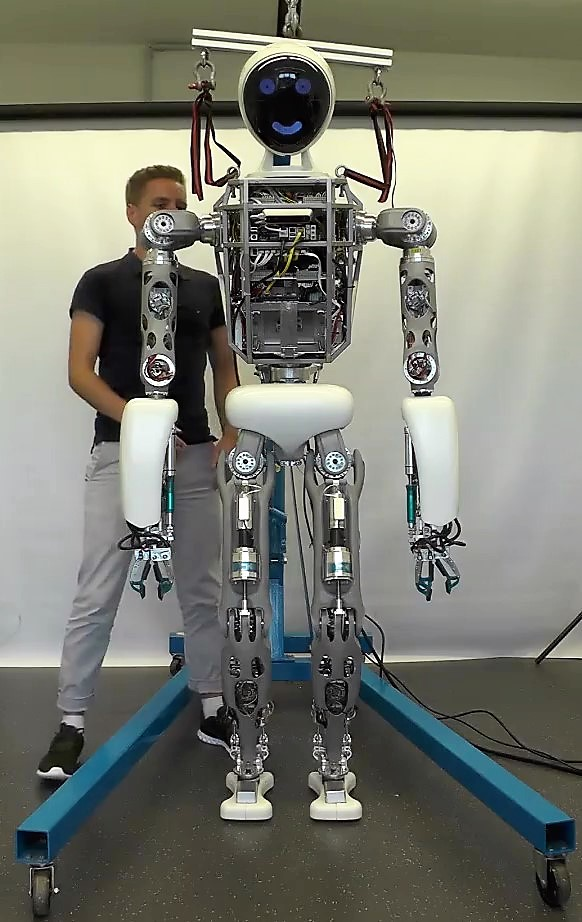
\includegraphics[width=.95\linewidth]{experiments/walkDynamic/snaps/1}
	\end{subfigure}%
\begin{subfigure}{.2\textwidth}
	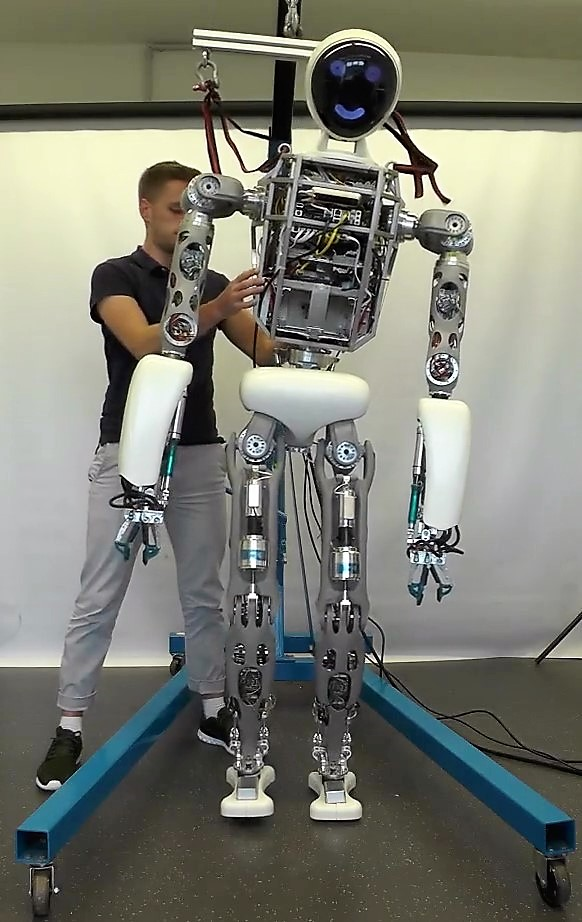
\includegraphics[width=.95\linewidth]{experiments/walkDynamic/snaps/2}
\end{subfigure}%
\begin{subfigure}{.2\textwidth}
	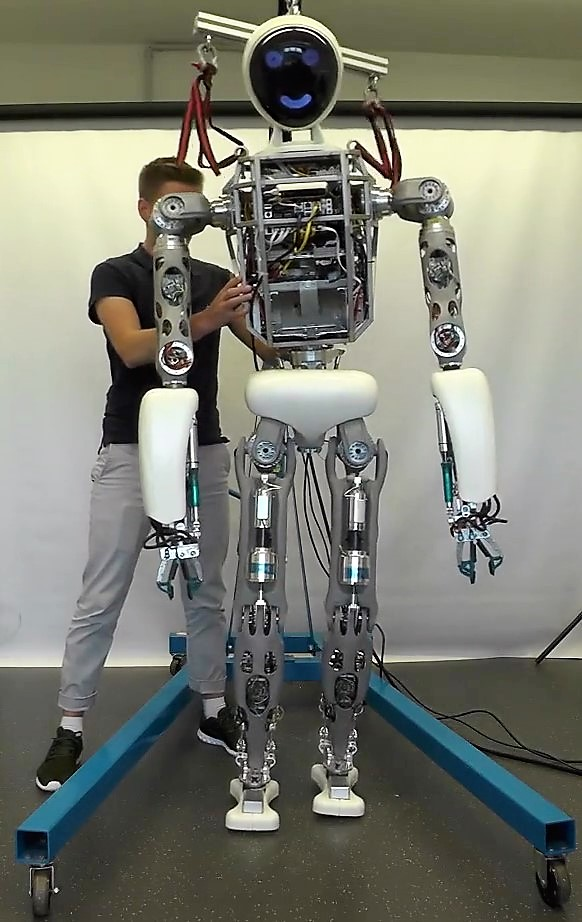
\includegraphics[width=.95\linewidth]{experiments/walkDynamic/snaps/3}
	\end{subfigure}%
\begin{subfigure}{.2\textwidth}
	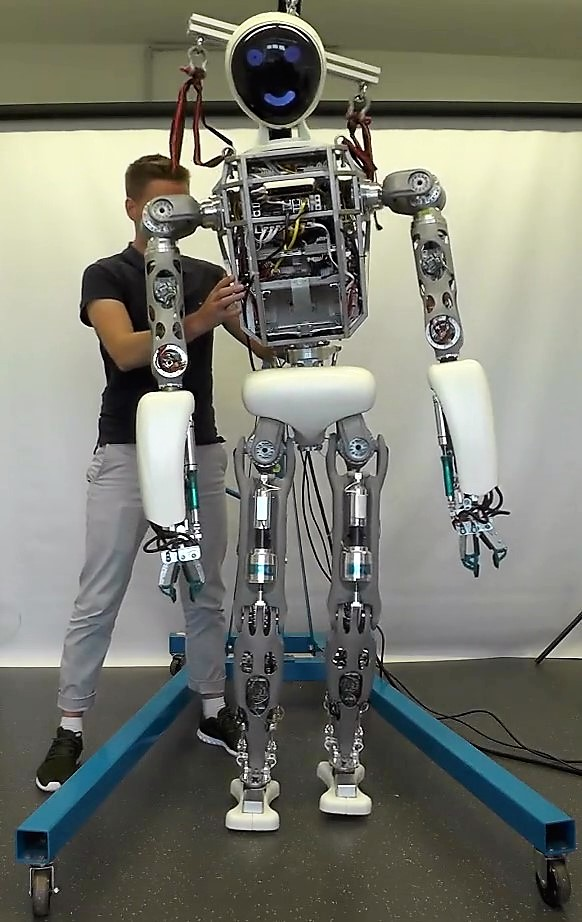
\includegraphics[width=.95\linewidth]{experiments/walkDynamic/snaps/4}
\end{subfigure}%
\begin{subfigure}{.2\textwidth}
	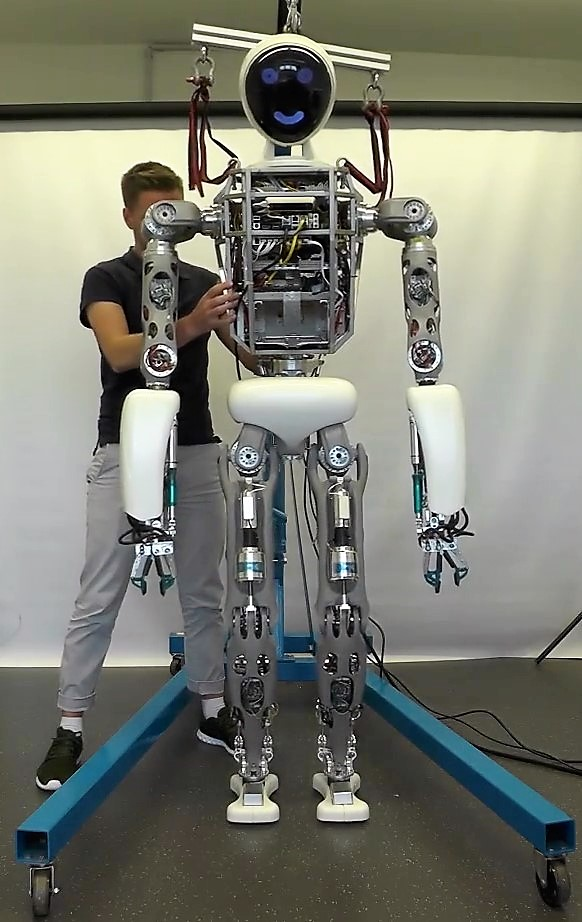
\includegraphics[width=.95\linewidth]{experiments/walkDynamic/snaps/5}
	\end{subfigure}%
\caption{Experiment IV: Dynamic walking.}
\label{exp:dynamicWalkingSnaps}
\end{figure} 

\subsection{Discussion}
The following section analyzes the experimental results, highlighting limits of the utilized control architecture.
\subsubsection{Stability of the Motions}
All in all, three out of four planned motions could be successfully stabilized by the  controller on the real system (see \cref{tab:experiments}). Both, the one-leg balancing experiment (I) and the fast squats experiment (III) were stabilized with good accuracy. For experiment II, static walking, only one step could be stabilized at a time. Furthermore it could be shown that dynamic walking (IV) cannot be stabilized with the present control approach. 
\subsubsection{Tracking Performance}
As detailed in \cref{subsec:Pipeline}, the online stabilizer solely works in joint space. The experimental results indicate that the overall joint space tracking for all four experiments is good. 
\cref{exp:BalancingTracking} exemplary shows the tracking performance for the one-leg balancing experiment. It becomes evident that the control architecture allows following the computed reference trajectory in actuator space (a,b) fairly well. Furthermore, also the resulting tracking quality in the virtual joints (c,d) is satisfying. Similar conclusions hold for the other experiments. Even during critical impulse phases the joint space tracking shows no abnormalities. This good tracking is achieved with high-gain joint space control, which allows a quick compensation of position differences that comes at the cost of lost compliance in the joints.
\begin{figure}[h!]
\begin{subfigure}{.5\textwidth}
	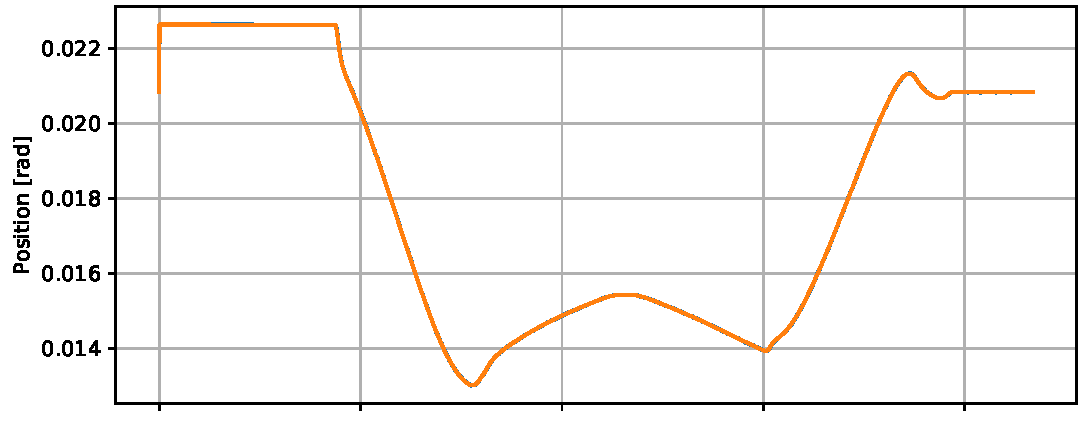
\includegraphics[page=1, width=.95\linewidth]{experiments/balancing/ankleTrack}
	\caption{LLAnkleAct1}	
	\end{subfigure}%
\begin{subfigure}{.5\textwidth}
	\includegraphics[page=2, width=.95\linewidth]{experiments/balancing/ankleTrack}
	\caption{LLAnkleAct2}	
\end{subfigure}%

\begin{subfigure}{.5\textwidth}
	\includegraphics[page=3, width=.95\linewidth]{experiments/balancing/ankleTrack}
	\caption{LLAnkleRoll}	
	\end{subfigure}%
\begin{subfigure}{.5\textwidth}
	\includegraphics[page=4, width=.95\linewidth]{experiments/balancing/ankleTrack}
	\caption{LLAnklePitch}	
\end{subfigure}%
\caption{Tracking performance for the one-leg balancing experiment in actuator space (a,b) and independent joint space (c,d). The reference position from \gls{OC} in orange and the measured position in blue are plotted against the time.}
\label{exp:BalancingTracking}
\end{figure} 
\subsubsection{Handling Impulses}
The impact phase turned out to be the main problem for the walking experiments. This is reasonable since the utilized control approach only compensates for errors in joint space, while errors in tasks space can arise quickly and are not compensated. Deviations of the reference base motion only effect the static stability if the \gls{FCoM} leaves the support polygon. Differences from the foot position instead, may cause instability with an respective error in the range of a few millimeters. The same holds for errors in the foot orientation. Consider for example the case where the robot only touches the ground with the rear part of the swing foot's sole. Instead of the assumed surface contact between the foot and the ground, a line contact appears that causes the robot to fall in a combination with high-gain position control. 
\subsubsection{Model Discrepancies}
The quasi-static experiments provide a good basis of analyzing the model accuracy. Due to the small \gls{SP}, model deviations inevitably lead to instability during the single support phases. In the balancing and static walking experiments the motions could be stabilized if, and only if, the \gls{FCoM} was adjusted by about $\pm$ 7.5mm. The found model errors in the mass distribution, eventually combined with with errors in inertia distribution, may also pose part of the problem for walking gait stabilization. In order to compensate for these differences, an extensive system identification could be performed to check the dynamic model against the real system.
\subsubsection{Mechanical Deficiencies}
Beneath the identified limits of the control approach and the modeling errors, also mechanical weaknesses of the RH5 humanoid may contribute to the sim-to-real gap. In the scope of the experiments, several issues have been revealed, namely joint play, calibration errors and undesired structural flexibility in the ankle of the foot. Furthermore, the rigid contact points on the sole of the feet are found to be not the ideal solution, since also small deviations can quickly lead to instability of the whole system. Instead, it may be advantageous for dynamic movements of the humanoid robot to use a planar sole, providing adequate damping properties. 


























